\section{PDF space estimators}

\begin{itemize}
    \item Covmat becomes unstable if Nx is increased beyond 4
    \item diagonal xi and ratio agree and look good for nx = 4
    \item x basis xi can still be calculated for any nx, we find it to
        be very stable, look pretty good and agree with low Nx diagonal result
\end{itemize}

We can calculate the same set of estimators in PDF space with minor alteration
to the definitons. Firstly, we are free to choose our own data points which will
be points in x and flavour for the PDFs at the initial scale. For this study the
points in x for singlet and gluon were chosen to be half logarithmically spaced
between $10^-3<x<0.1$ and half linearly spaced between $0.1<x<0.5$. For the
other flavours (V, V3, V8, T3, and T8) we simply choose the points to be
linearly spaced $0.1<x<0.5$ which is supposed to roughly capture the data
region of the PDFs.

The covariance matrix which is used in the definition
of bias and variance is estimated from the union of all of the replicas, allowing
for correlations across different flavours. We can also calculate $\xi_{1\sigma}$
in the basis which diagonalises this covariance matrix and show that this gives
much good agreement between the expected $\xi_{1\sigma}$ and that measured
directly from the PDFs.

\subsection{Stability of estimated covariance matrix}

Before looking at the estimators, it's useful to see how stable the covariance
matrix estimated from the PDF replicas is under variations of the number of x
points for each flavour. We show the eigenvalues of the correlation matrices
for $N_x = 4,\,6\,8$ and $12$. We see that the l2-condition number of the
correlation matrix starts to increase with $N_x$ rapidly even between $N_x=4$
and $N_x=6$. This leads us to conclude that bias, variance and $\xi_{1\sigma}$
in the basis which diagonalises the covariance matrix might have reliability
issues beyond $N_x = 4$ because the amount of statistics to accurately
calculate the covariance matrix becomes much greater.

EIGENVAL PLOTS

\subsection{Results for $N_x=4$}

SQRT RATIO

XI

\subsection(Results in x-basis)

Alternatively we can try calculating $\xi_{1\sigma}$ in the x-basis and ignore
any correlations. This still will give an indication of whether the distribution
at each point in x is similar between the PDF replicas for a given fit and the 
expectation of the PDF replicas at each point in x across fits. Since there
is no covariance matrix calculation we are free to increase the number of points
in x, with the caveat that the average of $\xi_{1\sigma}^i$ across x values
becomes the average of an increasingly correlated sample of points. Something
which is quite reassuring is that the $\xi_{1\sigma}$ is stable under variations
of $N_x$.

First the ratio of bias/variance for each flavour and total.

\begin{center}
    \begin{tabular}{lr}
        \toprule
        {} &  bias/variance \\
        flavour  &                \\
        \midrule
        $\Sigma$ &           0.58 \\
        gluon    &           0.90 \\
        V        &           0.73 \\
        V3       &           0.77 \\
        V8       &           0.62 \\
        T3       &           0.33 \\
        T8       &           1.18 \\
        Total    &           0.66 \\
        \bottomrule
        \end{tabular}
\end{center}

Now we compare the measured $\xi_{1\sigma}$ with the expected $\xi_{1\sigma}$
calculated from bias/variance.

\begin{center}
    \begin{tabular}{lrr}
        \toprule
        {} &  Measured $\xi_{1\sigma}$ & expected $\xi_{1\sigma}$ from bias/variance \\
        flavour  &                           &                           \\
        \midrule
        $\Sigma$ &                      0.78 &                      0.81 \\
        gluon    &                      0.68 &                      0.71 \\
        V        &                      0.76 &                      0.76 \\
        V3       &                      0.69 &                      0.75 \\
        V8       &                      0.80 &                      0.80 \\
        T3       &                      0.91 &                      0.92 \\
        T8       &                      0.60 &                      0.64 \\
        Total    &                      0.79 &                      0.78 \\
        \bottomrule
        \end{tabular}
\end{center}

For each flavour we can plot $\xi^{i}_{1\sigma}$, the contribution to $\xi_{1\sigma}$
from each of eigenvectors

\begin{figure}
    \centering
    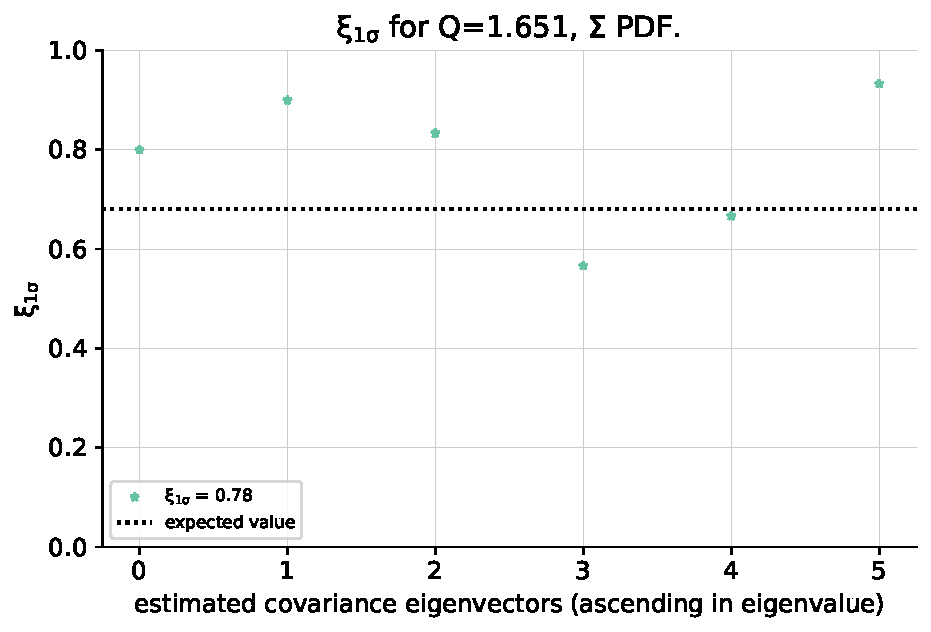
\includegraphics[width=0.6 \textwidth]{diag_sigma.pdf}
    \caption{
        $\xi^{i}_{1\sigma}$ for singlet PDF, in the basis which diagonalises
        the covariance matrix, estimated from the union of all the replicas
    }
    \label{fig:pdfdiagsinglet}
\end{figure}

\begin{figure}
    \centering
    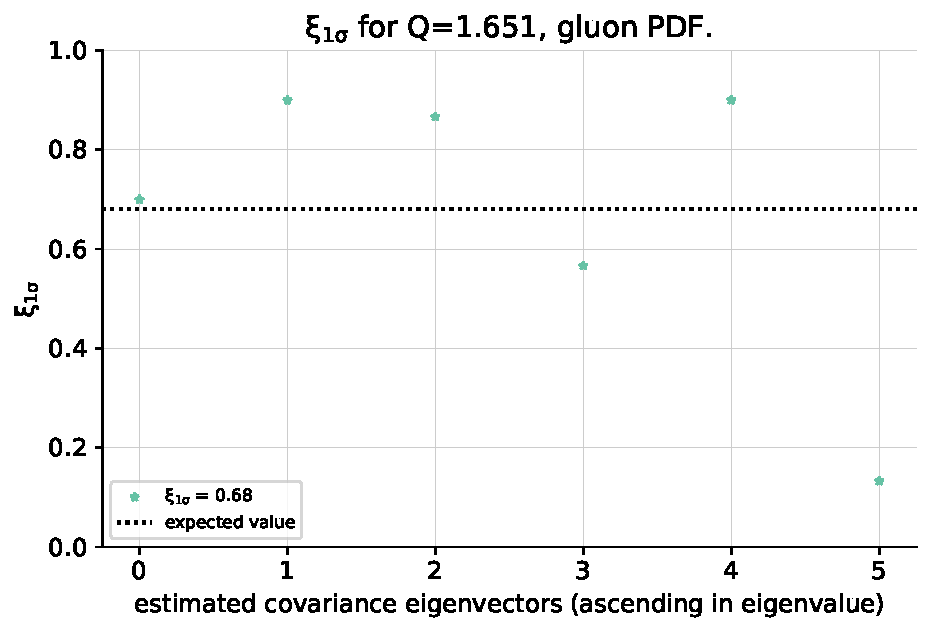
\includegraphics[width=0.6 \textwidth]{diag_gluon.pdf}
    \caption{
        $\xi^{i}_{1\sigma}$ for gluon PDF, in the basis which diagonalises
        the covariance matrix, estimated from the union of all the replicas
    }
    \label{fig:pdfdiaggluon}
\end{figure}

\begin{figure}
    \centering
    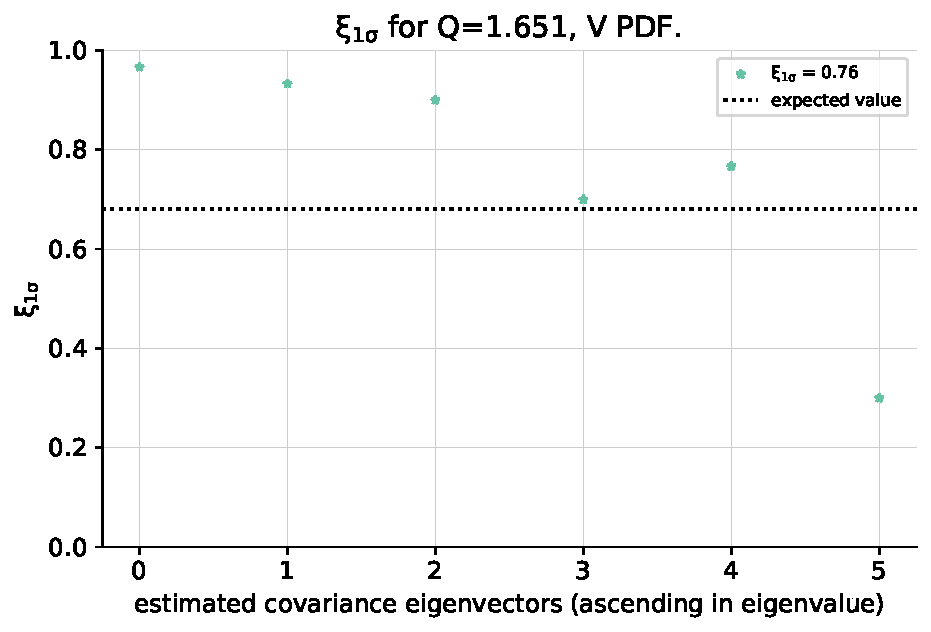
\includegraphics[width=0.6 \textwidth]{diag_v.pdf}
    \caption{
        $\xi^{i}_{1\sigma}$ for V PDF, in the basis which diagonalises
        the covariance matrix, estimated from the union of all the replicas
    }
    \label{fig:pdfdiagv}
\end{figure}

\begin{figure}
    \centering
    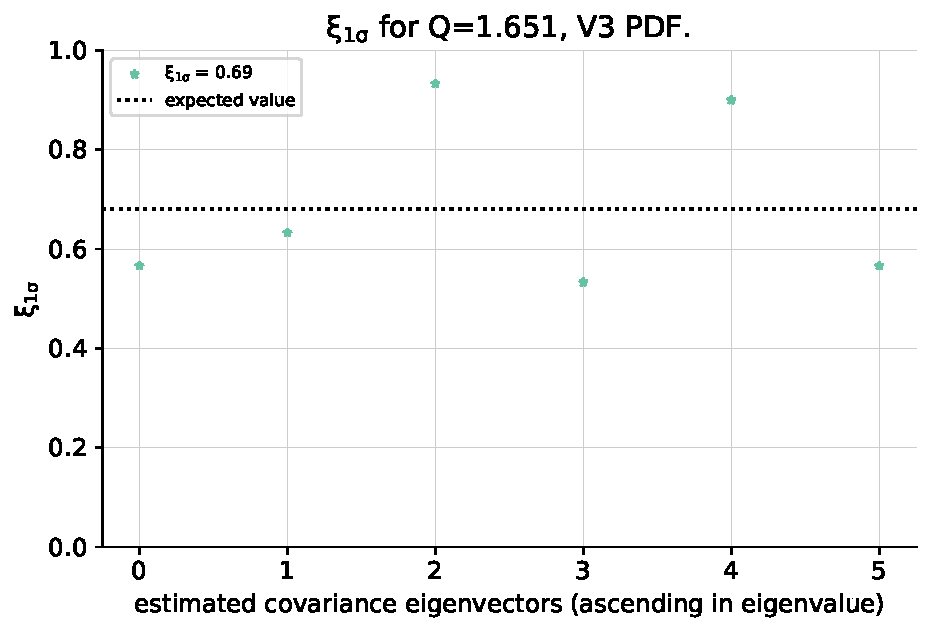
\includegraphics[width=0.6 \textwidth]{diag_v3.pdf}
    \caption{
        $\xi^{i}_{1\sigma}$ for V3 PDF, in the basis which diagonalises
        the covariance matrix, estimated from the union of all the replicas
    }
    \label{fig:pdfdiagv3}
\end{figure}

\begin{figure}
    \centering
    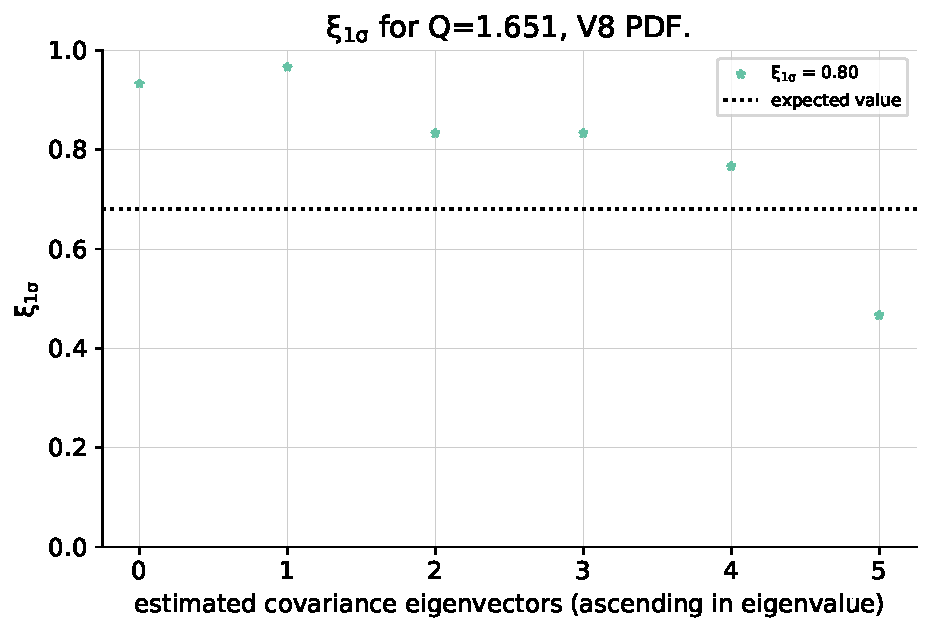
\includegraphics[width=0.6 \textwidth]{diag_v8.pdf}
    \caption{
        $\xi^{i}_{1\sigma}$ for V8 PDF, in the basis which diagonalises
        the covariance matrix, estimated from the union of all the replicas
    }
    \label{fig:pdfdiagv8}
\end{figure}

\begin{figure}
    \centering
    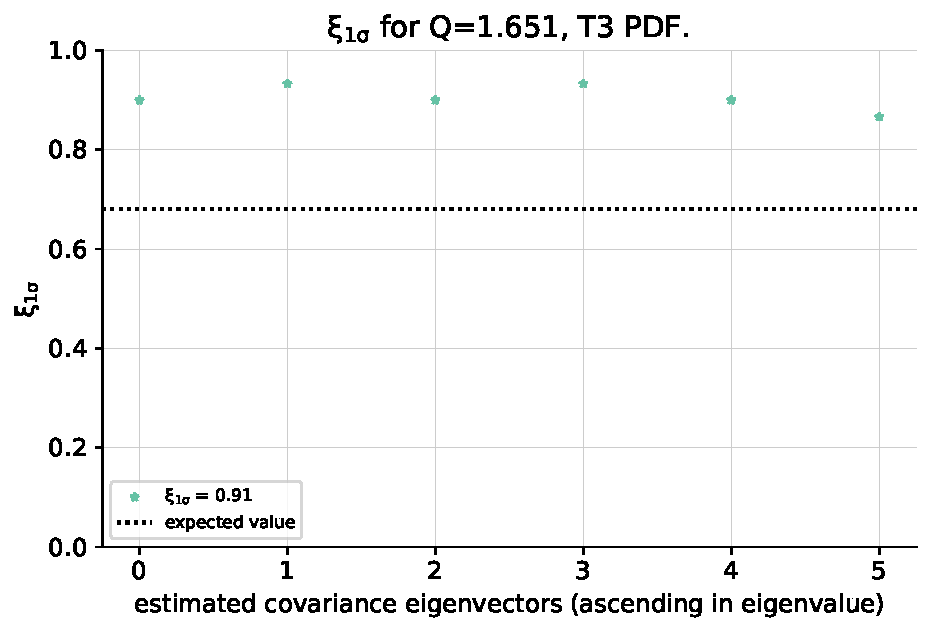
\includegraphics[width=0.6 \textwidth]{diag_t3.pdf}
    \caption{
        $\xi^{i}_{1\sigma}$ for T3 PDF, in the basis which diagonalises
        the covariance matrix, estimated from the union of all the replicas
    }
    \label{fig:pdfdiagt3}
\end{figure}

\begin{figure}
    \centering
    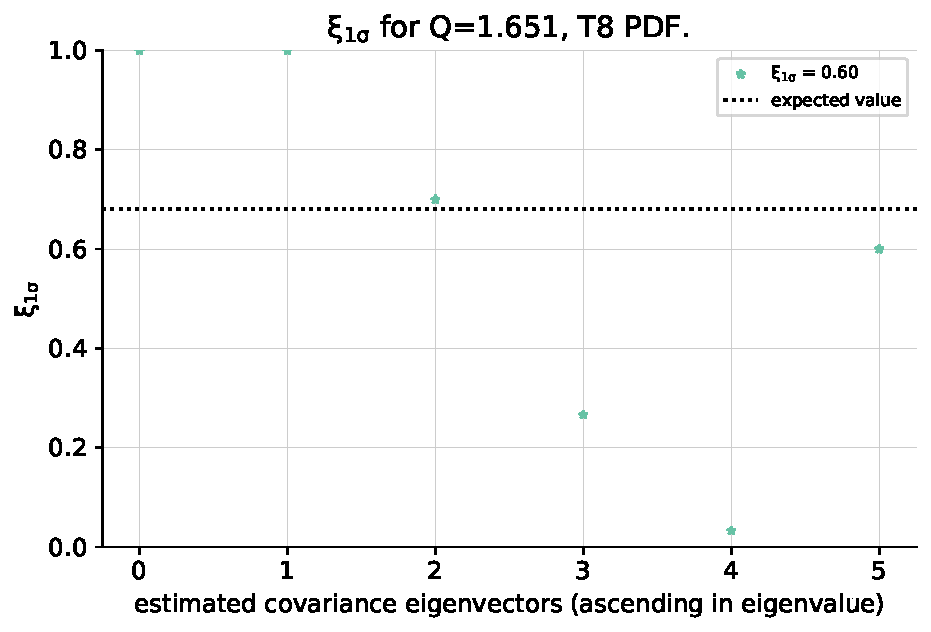
\includegraphics[width=0.6 \textwidth]{diag_t8.pdf}
    \caption{
        $\xi^{i}_{1\sigma}$ for T8 PDF, in the basis which diagonalises
        the covariance matrix, estimated from the union of all the replicas
    }
    \label{fig:pdfdiagt8}
\end{figure}

The PDF results are highly dependent on the number of points chosen in x. Also
the results in the basis which diagonalise the covariance matrix stop us from
seeing how the results depend on x, with the benefit of $\xi_{1\sigma}$ and
the expected results from bias/variance agreeing well. Potentially a far greater
number of fits and replicas are required to get a more reliable result, however
the numbers in the first and second table don't look too bad.
